% 3-var K-map for the alarm: I&D | I&~B -> I&D + I&~B
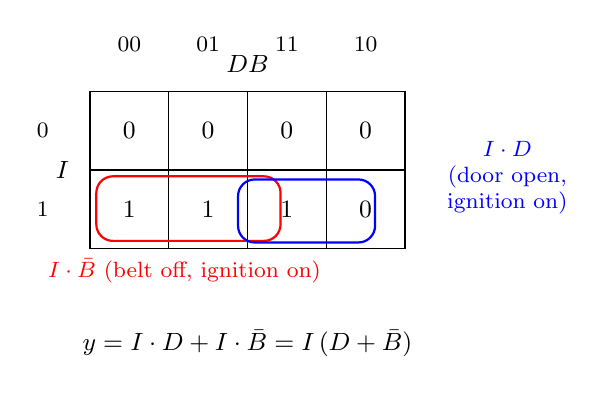
\begin{tikzpicture}[font=\small]
\draw[step=1] (0,0) grid (4,2);
\node at (-0.35,1.0) {$I$}; \node at (2.0,2.35) {$DB$};
\node[font=\footnotesize] at (-0.6,1.5) {0}; \node[font=\footnotesize] at (-0.6,0.5) {1};
\node[font=\footnotesize] at (0.5,2.6) {00}; \node[font=\footnotesize] at (1.5,2.6) {01};
\node[font=\footnotesize] at (2.5,2.6) {11}; \node[font=\footnotesize] at (3.5,2.6) {10};
% I row (bottom, I=1): DB cols 00->1, 01->1, 11->1, 10->0
\node at (0.5,0.5) {1}; \node at (1.5,0.5) {1}; \node at (2.5,0.5) {1}; \node at (3.5,0.5) {0};
\node at (0.5,1.5) {0}; \node at (1.5,1.5) {0}; \node at (2.5,1.5) {0}; \node at (3.5,1.5) {0};
\draw[red, thick, rounded corners=6pt] (0.08,0.10) rectangle (2.42,0.92);
\node[red, font=\footnotesize] at (1.2,-0.28) {$I\cdot\bar B$ (belt off, ignition on)};
\draw[blue, thick, rounded corners=6pt] (1.88,0.08) rectangle (3.62,0.88);
\node[blue, font=\footnotesize, align=center] at (5.3,0.9) {$I\cdot D$\\ (door open,\\ ignition on)};
\node at (2.0,-1.2) {$y = I\cdot D + I\cdot\bar B = I\,(D+\bar B)$};
\end{tikzpicture}
